\documentclass[a4paper,11pt]{article}
\usepackage[utf8]{inputenc}
\usepackage{subfigure}
\usepackage{rotating}
\usepackage{nicefrac}
\usepackage{float}
\usepackage{amsmath}
\usepackage{amssymb}
\usepackage{hyperref}
\usepackage[export]{adjustbox}
\usepackage[T1]{fontenc}
\usepackage{enumitem}
\usepackage{lstautogobble}		% Pour mettre à gauche le code
\usepackage{listings}			% Pour afficher du code
\usepackage{graphicx} 			% Pour l'affichage d'images
\usepackage{titling} 			% Reduit l'espace au dessus du titre et auteurs
\usepackage[left=20mm,top=10mm, right=18mm, bottom=10mm, includefoot]{geometry}

\title{\textsc{[INFO-H-303] Bases de données - Rapport Projet:}\
   "Ebay"}
\author{Alexandre Heneffe - 000440761\\
        Nicolas Jonas - 000442112\\
        Evgueniy Starygin - 000443325}
\date{Mars 2018}

\begin{document}
\maketitle
\section{Introduction}

Ceci est le rapport du projet de base de données. Celui-ci contiendra le schéma entité-relationnel (et ses contraintes) de la future base de données ainsi que sa traduction en un modèle relationnel.

\subsection{Hypothèses}

\begin{itemize}[label=\textbullet]
	\item Un objet appartient à 1 catégorie
	\item Une catégorie peut exister sans objet y étant associé
	\item Chaque objet est unique, il n'y a pas de notion de quantité
	\item Un utilisateur doit être majeur afin d'acheter des objets

\end{itemize}

\subsection{Contraintes d'intégrités}

\begin{itemize} [label=\textbullet]
	\item La date de vente d'un objet doit être > à la date de mise en vente de cet objet
	\item Le prix proposé pour une proposition d'achat doit être >= au prix minimum de l'objet
	\item Un administrateur ne peut pas se supprimer lui-même
	\item L'évaluation d'un objet est faite que si cet objet est acheté depuis moins de 10 jours, c'est-à-dire que la date d'évaluation doit être < à
	la date de vente de l'objet + 10
	\item La date d'évaluation d'un objet doit être > à la date de vente d'un objet
	\item Le pseudo d'un utilisateur est unique (c'est ce qui permet de différencier les utilisateurs)
	\item Le vendeur d'un objet ne peut pas être l'acheteur de cet objet
	\item la date de naissance d'un vendeur doit être > à la date de mise en vente d'un objet qu'il vend
	\item la note d'une évaluation est une valeur entre 1 et 10
	\item le numéro d'une évaluation doit être unique
	
\end{itemize}

\section{Modèle Entité-Association}
\subsection{Schéma}
\begin{center}
  \begin{sidewaysfigure}
    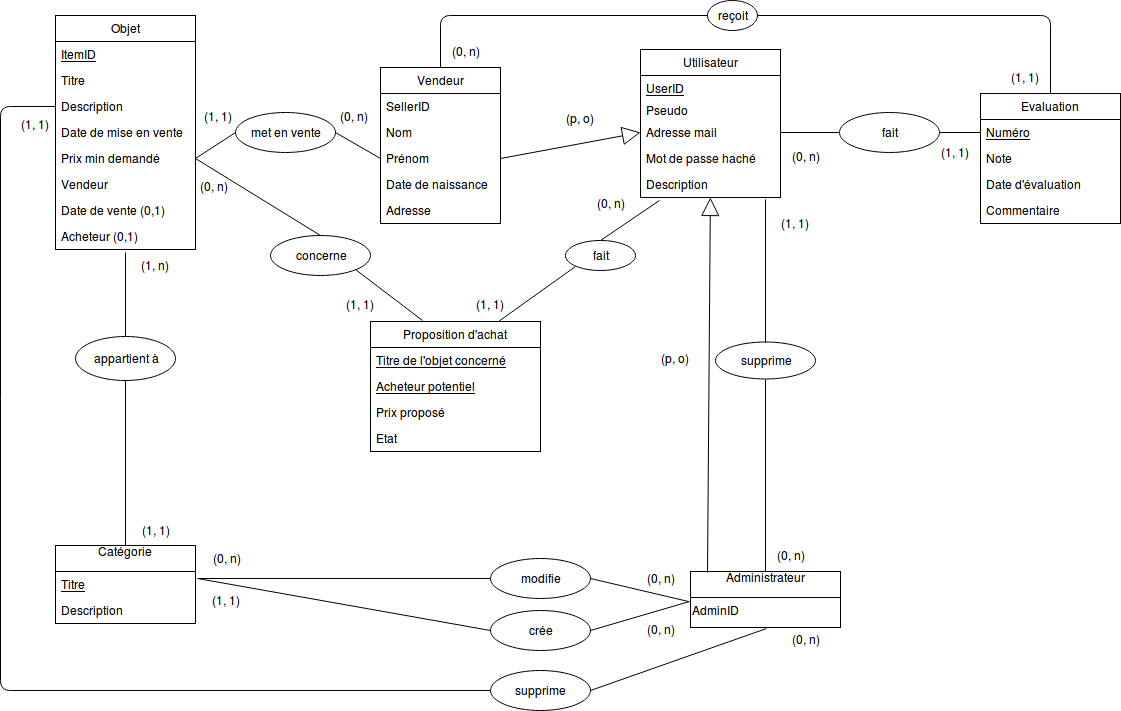
\includegraphics[width = 25cm]{SchemaEA.png}
  \end{sidewaysfigure}
\end{center}

\newpage

\subsection{Justifications}
La généralisation (Utilisateur, vendeur et administrateur) dans le schéma, est partiel et couvrant.
\begin{itemize}
\item Partiel: Les vendeurs et administrateurs sont des types d'utilisateurs. Mais il y a aussi les utilisateurs classiques.
\item Couvrant: Un utilisateur peut être à la fois vendeur et administrateur par exemple.
\end{itemize}

\textbf{Evaluations :} une évaluation a pour clef un Numéro (qui doit donc être unique) car ses autres attributs ne permettent pas de la
	      distinguer de manière unique (ex : deux évaluations peuvent avoir la même note et la même date).

\textbf{Utilisateur :} un utilisateur quelque soit son statut (simple utilisateur, vendeur et/ou administrateur) reste toujours identifié
par son Pseudo.

\textbf{Proposition d'achat :} un proposition d'achat est identifiée à la fois par le Titre de l'objet concerné et par l'Acheteur potentiel,
car on ne peut se baser uniquement sur le Titre de l'objet (il peut y avoir plusieurs propositions d'achat pour un même objet)
ou sur le Pseudo de l'acheteur potentiel (un acheteur peut faire plusieurs propositions d'achats sur différenets Objets).

\section{Modèle Relationnel}
Dans cette section, nous traduisons le modèle entité-association de la section précédente en un modèle relationnel et en ajoutant ses contraintes.

\subsection{Modèle}

\indent

\subsubsection{Utilisateur}
\fbox{\underline{UserID} | MotDePasse | Pseudo | AddresseMail | Description}\\


\subsubsection{Administrateur}
\fbox{\underline{AdminID}}\\ \\
\indent - Administrateur.AdminID référence Utilisateur.UserID \\
\indent \indent $\rightarrow$ L'administrateur est une généralisation de l'utilisateur, il en hérite


\subsubsection{Vendeur} 
\fbox{\underline{SellerID} | Nom | Prénom | DateNaissance | Adresse}\\ \\
\indent - Vendeur.SellerID référence Utilisateur.UserID \\
\indent \indent $\rightarrow$ Le vendeur est une généralisation de l'utilisateur, il en hérite


\subsubsection{Catégorie}
\fbox{\underline{Titre} | Description\_cat | AdminID}\\ \\
\indent - Catégorie.AdminID référence Administrateur.AdminID\\
\indent \indent $\rightarrow$ Une catégorie est créée par (1,1) administrateur


\subsubsection{Objet}
\fbox{\underline{ItemID} | Titre | Description\_obj | DateMiseEnVente | PrixMin | DateVente | Acheteur | SellerID |  Categorie}\\ \\
\indent - Objet.SellerID référence Vendeur.SellerID \\
\indent \indent $\rightarrow$ Un objet est mis en vente par (1,1) vendeur\\
\indent - Objet.Categorie référence Categorie.Titre \\
\indent \indent $\rightarrow$ Un objet appartient à (1,n) catégories


\subsubsection{Evaluation}
\fbox{\underline{Numéro} | Buyer | Seller | Time | Rate | Commentaire}\\ \\
\indent - Evaluation.Seller référence Vendeur.SellerID\\
\indent \indent $\rightarrow$ une evaluation est reçue par (1,1) vendeur\\
\indent - Evaluation.Buyer référence Utilisateur.UserID\\
\indent \indent $\rightarrow$ une evaluation est faite par (1,1) utilisateur


\subsubsection{PropositionAchat}
\fbox{\underline{ItemID} | Time | Buyer | price | accepted}\\ \\
\indent - PropositionAchat.ItemID référence Objet.ItemID \\
\indent \indent $\rightarrow$ Une proposition d'achat est concernée par (1,1) objet\\
\indent - PropositionAchat.Buyer référence Utilisateur.UserID \\
\indent \indent $\rightarrow$ Une proposition d'achat est faite par (1,1) utilisateur



\subsection{Contraintes d'intégrité}

\begin{itemize}
    \item Pour tout Objet.Titre, il existe au moins un Appartenance.TitreObj
    \item Pour un Objet, Objet.DateVente > Objet.DateMiseEnVente
    \item Pour un PropositionAchat, PropositionAchat.Prix >= Objet.PrixMin
    \item Pour un Utilisateur, Administrateur.Pseudo != Utilisateur.Pseudo (un Administrateur ne peut pas se supprimer)
    \item Pour un Evaluation, Evaluation.Date < Objet.DateVente + 10
    \item Pour un Evaluation, Evaluation.Date > Objet.DateVente
    \item Pour un Vendeur, Vendeur.DateNaissance >= 18
    \item Pour un Vendeur, Vendeur.DateNaissance > Objet.DateMiseEnVente
    \item Pour un Objet, Objet.Vendeur != Objet.Acheteur
\end{itemize}

\section{Gestion des données}

Explications des méthodes utilisées pour l'extraction des données

Pour insérer les données des fichiers dans la base de données, nous avons utilisé la commande "LOAD DATA LOCAL INFILE" pour les fichiers .txt et la commande "LOAD DATA LOCAL INFILE" pour les fichiers .xml. 

\section{Requêtes demandées}

\subsection{R1}

$\rightarrow$ Les vendeurs qui sont appréciés par les utilisateurs ayant les memes
gouts que l'utilisateur 'Jules'. Les goûts d'un utilisateur' sont définis par les vendeurs auxquels cet utilisateur a donné une évaluation supérieure (ou égale) à 3 sur 5.

\subsubsection{SQL}

SELECT DISTINCT v1.SellerID
FROM Vendeur v1, Evaluation e1, Utilisateur u1\\
WHERE e1.Seller = v1.SellerID AND u1.UserID = e1.Buyer AND e1.Rate >= 3 AND u1.UserID in \\
\indent \indent SELECT u2.UserID \\
\indent \indent FROM Vendeur v2, Evaluation e2, Utilisateur u2 \\
\indent \indent WHERE u2.UserID = e2.Buyer AND v2.SellerID = e2.Seller \\
\indent \indent AND e2.Rate > 3 AND v2.SellerID in \\
\indent \indent \indent \indent SELECT v3.SellerID\\
\indent \indent \indent \indent FROM Vendeur v3, Utilisateur u3, Evaluation e3\\
\indent \indent \indent \indent WHERE e3.Seller = v3.SellerID AND e3.Buyer = u3.UserID\\
\indent \indent \indent \indent AND u3.UserID = 41 AND e3.Rate > 3))

\subsubsection{Algèbre relationnel}

$JulesID \leftarrow \pi_{SellerID} ( \sigma_{Prenom=``Jules''} (Vendeur)) $ \\
$SellerIDLikedByJules \leftarrow \pi_{SellerID}(\sigma_{Buyer=JulesID \wedge Rate \geq 3} (Evaluation))$\\
$BuyerWhoLikeAsJules \leftarrow \pi_{Buyer}(\sigma_{Rate \geq 3}(Evaluation *_{Seller=SellerID} LikedByJules))$\\
$R1 \leftarrow \pi_{SellerID}(\sigma_{Rate \geq 3}(BuyerWhoLikeAsJules*Evaluation))$

\subsubsection{Calcul tuple}

\{v2.SellerID | Vendeur(v2) $\land$ Evaluation(e3) $\land$ Vendeur(v) $\land$ v.Prenom = "Jules" $\land$\\
$\forall$u (Utilisateur(u) $\land$ \\
$\exists$e1 $\exists$e2 $\exists$v1 (Evaluation(e1) $\land$ Evaluation(e2) $\land$ Vendeur(v1)
$\land$ v1.SellerID = e1.Seller $\land$ \\v1.SellerID = e2.Seller $\land$
e1.Buyer = u.UserID $\land$ e2.Buyer = v.SellerID
$\land$ e1.Rate >= 3 $\land$ \\ e2.Rate >= 3)
$\rightarrow$ e3.Buyer = u.UserID $\land$ e3.Seller = v2.SellerID) \}


\subsection{R2}
$\rightarrow$ Les vendeurs ayant vendu et acheté à la meme personne

\subsubsection{SQL}

SELECT DISTINCT v.SellerID\\
FROM Vendeur v, Objet o1\\
WHERE v.SellerID = o1.SellerID AND o1.Acheteur IN\\
\indent \indent SELECT DISTINCT v2.SellerID\\
\indent \indent FROM Vendeur v2, Objet o2\\
\indent \indent WHERE v2.SellerID = o2.SellerID AND v.SellerID = o2.Acheteur)
    
\subsubsection{Algèbre relationnel}

$R2 \leftarrow \pi_{ItemID}((Objet \bowtie_{Buyer=Seller} \pi_{Seller,Buyer}(Objet)) 
			    \cap (Objet \bowtie_{Seller=Buyer} \pi_{Seller,Buyer}(Objet)))$

\subsubsection{Calcul tuple}

\{v.SellerID | Vendeur(v) $\land$ Objet(o1) $\land$ v.SellerID = o1.SellerID $\land$ $\exists$ v2 $\exists$ o2 (Vendeur(v2) $\land$ Objet(o2) $\land$ v2.SellerID = o2.SellerID $\land$ v.SellerID = o2.Acheteur $\land$ o1.Acheteur = v2.SellerID)\}


\subsection{R3}

$\rightarrow$ Les objets vendus à un prix inférieur au montant d'une proposition d'achat de cet objet

\subsubsection{SQL}

SELECT DISTINCT o.ItemID\\
FROM Objet o, PropositionAchat p\\
WHERE o.ItemID = p.ItemID AND p.accepted = 'True' AND\\
\indent \indent EXISTS (SELECT *\\
\indent \indent FROM PropositionAchat p1\\
\indent \indent WHERE p1.ItemID = p.ItemID AND p1.price > p.price AND p1.accepted = 'False')
        
\subsubsection{Algèbre relationnel}

$Vendus \leftarrow \pi_{ItemID, price}(\sigma_{accepted='True'}(PropositionAchat))$\\
$\alpha_{price:PrixVendu}(Vendus)$\\
$\alpha_{ItemID:ItemVenduID}(Vendus)$\\
$R3 \leftarrow \pi_{ItemID}(\sigma_{price \ln PrixVendu}(Vendus*_{ItemVenduID=ItemID}PropositionAchat)) $

\subsubsection{Calcul tuple}

\{o.ItemID | Objet(o) $\land$ PropositionAchat(p) $\land$ o.ItemID = p.ItemID $\land$ p.accepted = "True" $\land$ $\exists$p1 (PropositionAchat(p1) $\land$ p1.ItemID = p.ItemID $\land$ p1.price > p.price $\land$ p1.accepted = "False")\}
\subsection{R4}

$\rightarrow$ Le/Les vendeurs ayant vendu le plus d'objets dans la meme catégorie

\subsubsection{SQL}


\subsection{R5}

$\rightarrow$ Les objets pour lesquels au moins dix propositions d'achats ont été refusées

\subsubsection{SQL}

SELECT p.ItemID\\
FROM PropositionAchat p\\
WHERE p.accepted = "False"\\
GROUP BY p.ItemID\\
HAVING COUNT(*) >= 10

\subsection{R6}

$\rightarrow$ Les vendeurs avec le nombres moyen d'objets vendus, le nombre moyen d'objet achetés, la note qu'ils ont reçue, et la moyenne des notes qu'ils ont donné, et ce pour tous les vendeurs ayant vendu et acheté au moins 10 objets.

\subsubsection{SQL}


\section{Choix et hypothèses}

Explications et justifications des choix et hypothèses qu'on a pris

\begin{itemize}
	\item Pour la requête 1, on part du principe que si il y a ne serait ce qu'un meme élément en commun (vendeur apprécié), alors les 2 utilisateurs ont les memes gouts.
    \item Dans la table Administrateur, nous avons inséré un administrateur par défaut "Master" qui se chargera de créer les autres administrateurs.
    \item Nous avons décidé de ne pas stocker les suppressions et modifications faites par les administrateurs dans des tables dédiées.
   
    
\end{itemize}


\end{document}